\documentclass[aspectratio=169,11pt,svgnames]{beamer}

\usepackage[english]{babel}
\usepackage{graphicx}
\usepackage{enumitem}
\usepackage{amsmath}
\usepackage{mathtools}
\usepackage{float}
\usepackage{tikz}
\usetikzlibrary{patterns,arrows.meta}
\usepackage{tkz-euclide}
\tikzset{point style/.style = {%
  draw = black,
  inner sep = 0pt,
  shape = circle,
  minimum size = 5pt,
  fill = black
 }
}
\usepackage{enumitem}

\usepackage{caption}
\usepackage{subcaption}

% Flowchart stuff

\usepackage{pgfopts}
\usepackage{xcolor}
\usepackage{tcolorbox}

\usetheme[
 titlestyle=style2,
 titleformat=smallcaps,
 sectionstyle=plain,
 slidestyle=cyber,
 headingcolor=theme,
 block=transparent
]{trigon}

\title{Statistics}
\date{\today}
\author{Adam Klepáč}
\institute[GEVO]{Gymnázium Evolution Jižní Město}
\biglogo[width=.2\textwidth]{logo}
\smalllogo[width=.1\textwidth]{logo}
\titlegraphic{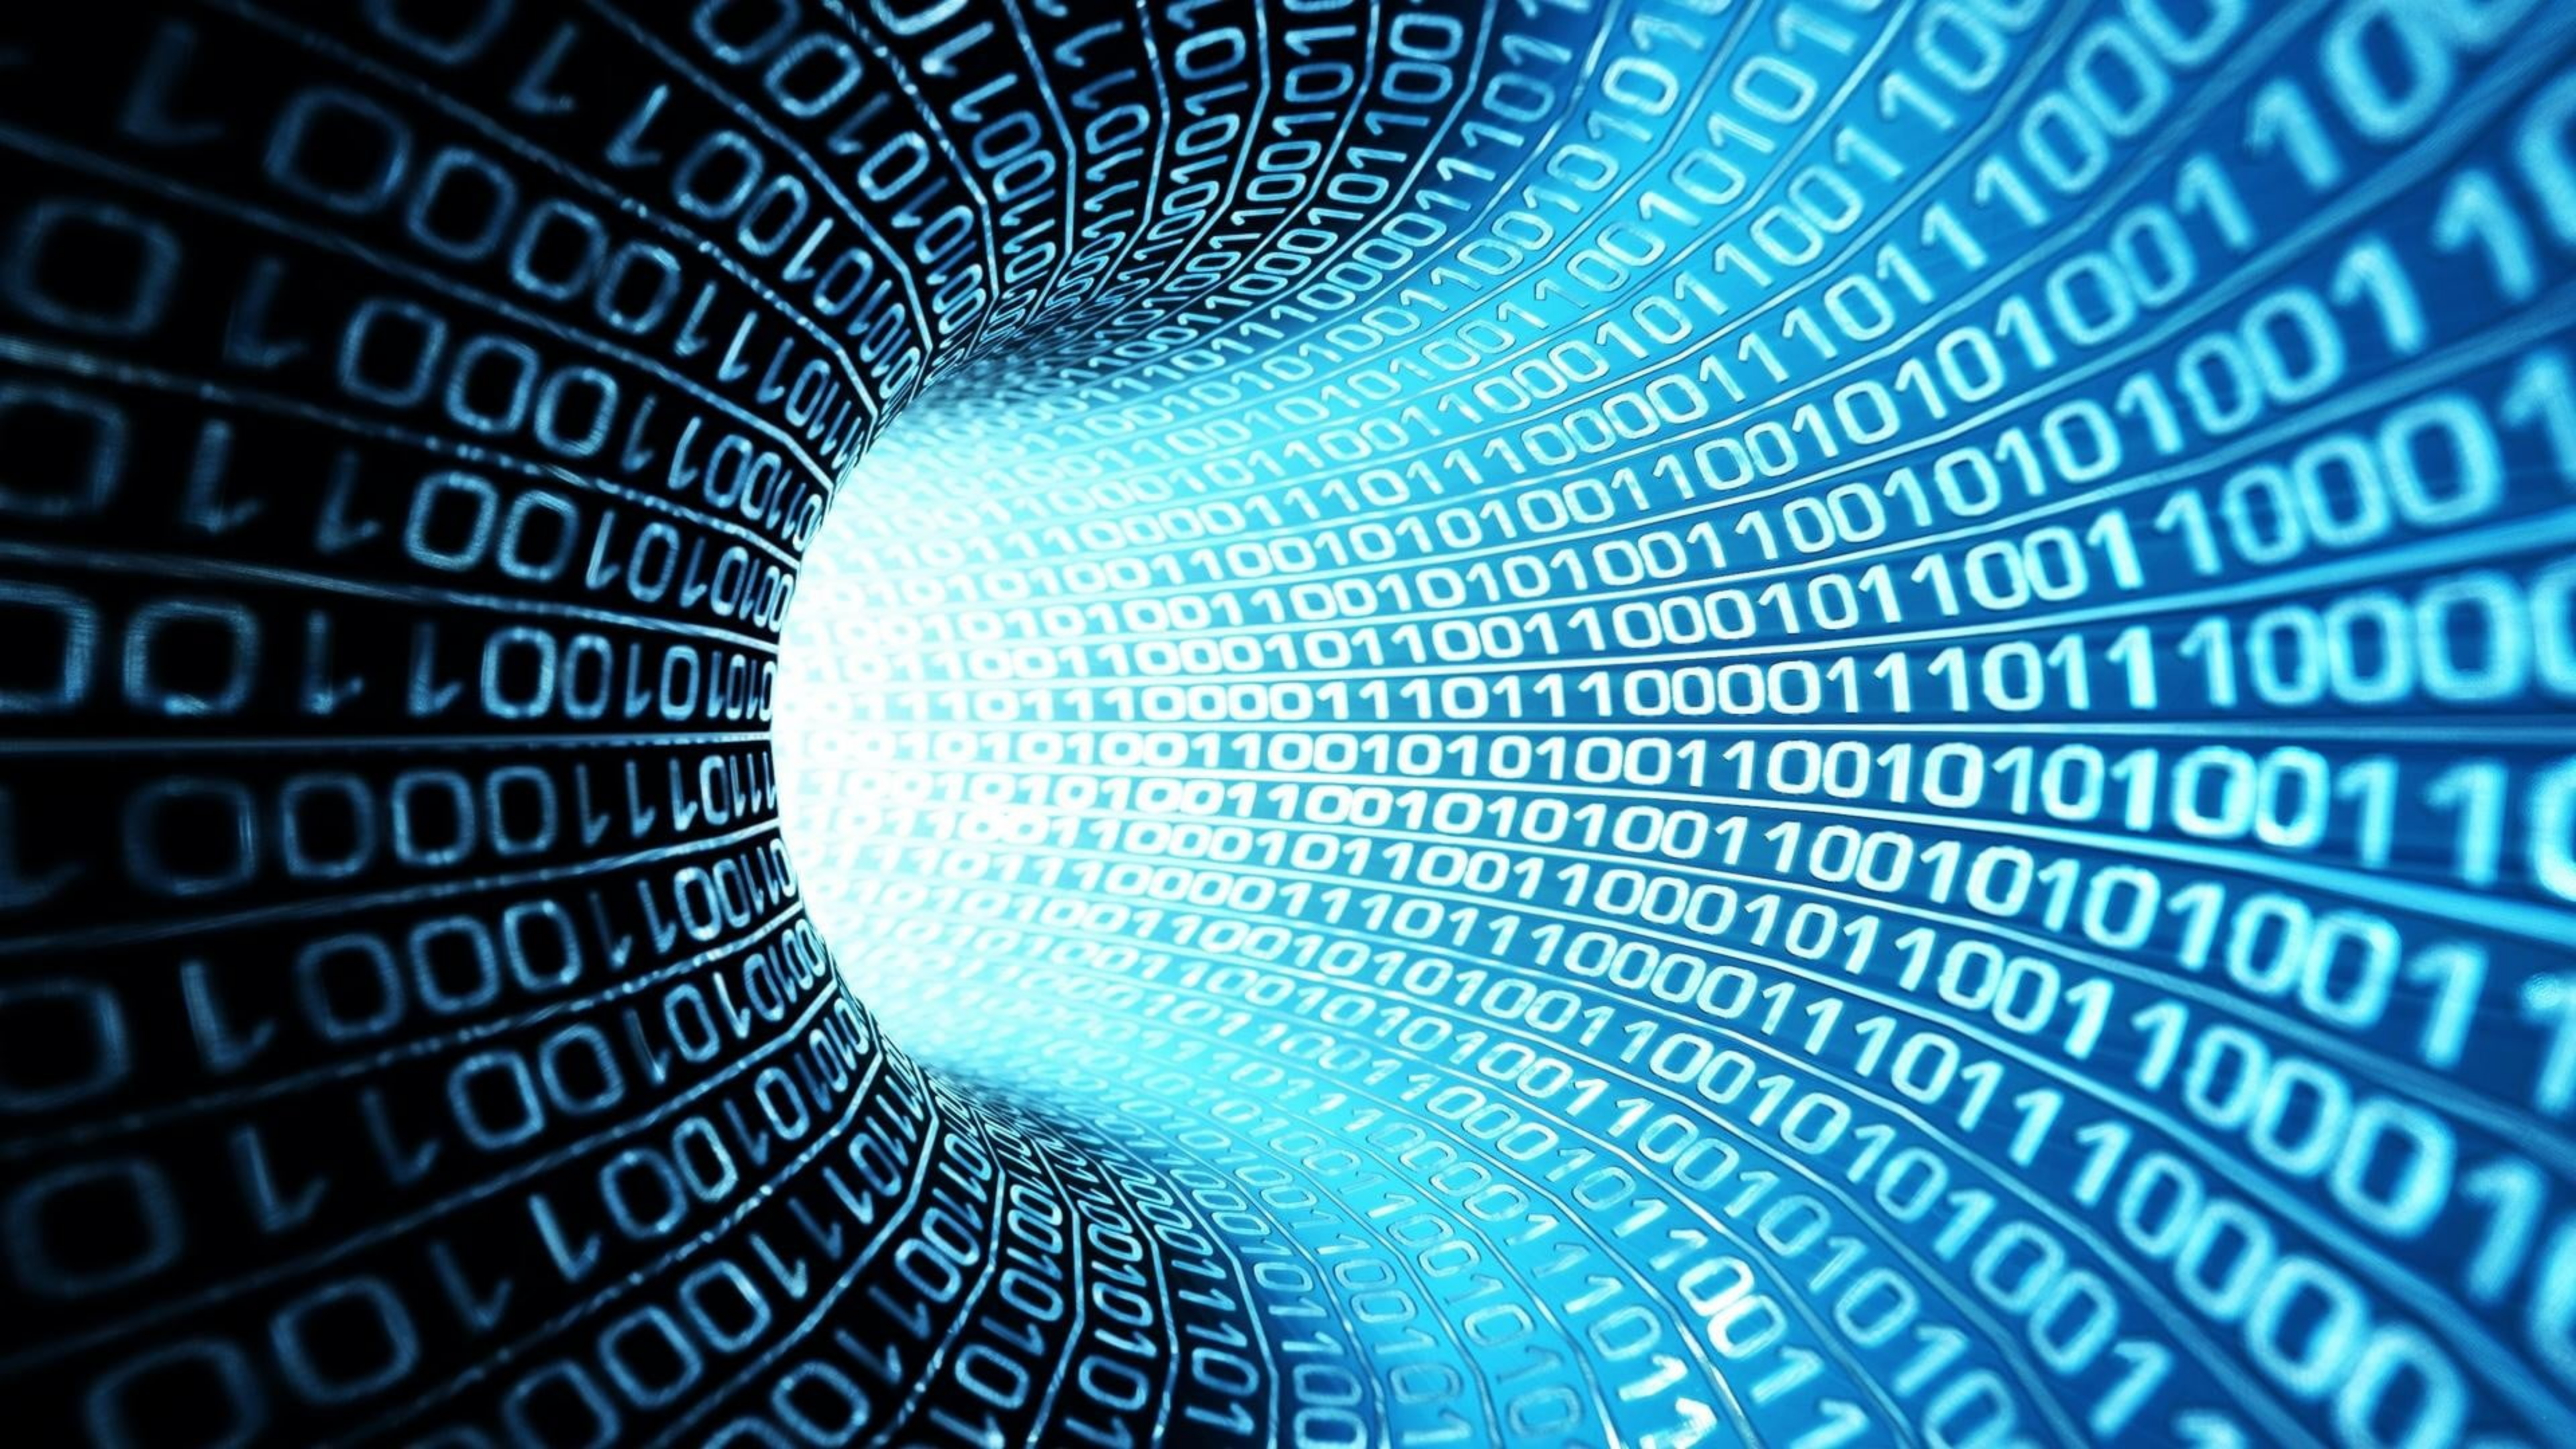
\includegraphics[height=\paperheight]{title.jpg}}

\def\subsectionname{}

% enumerate global settings
\setlist[enumerate,1]{label=\arabic*.}
\setlist[enumerate,2]{label=\alph*)}

% custom colors %
\definecolor{MyTeal}{HTML}{64CCC5}
\definecolor{MyNavy}{HTML}{053B50}
\definecolor{MyBlue}{HTML}{176B87}
\definecolor{MyWhite}{HTML}{EEEEEE}
\colorlet{tPrim}{MyTeal}
\colorlet{tTheme}{MyTeal}
\colorlet{tSec}{MyNavy}
\colorlet{tAccent}{MyBlue}

\tcbset{
 boxsep=7pt,
 fonttitle=\sc,
 colframe=tGreyBg,
 colframe=tPrim,
 boxrule=1pt
}

\begin{document}
\titleframe

\begin{frame}
 \frametitle{What Even Is Statistics?}
 \begin{tcolorbox}[title=Statistics]
  \alert{Statistics} is a mathematical discipline concerned with predicting
  future state of a system based \emph{solely} on its past behaviour.
 \end{tcolorbox}
 \pause
 The collective information about a system's past state is called
 \alert{data}.\\
 \pause
 It assigns \alert{probabilities} to each possible future state of system based
 on data.\\
 \pause
 It also assigns probabilities to the \alert{possibility of wrong prediction}.
\end{frame}

\begin{frame}
 \frametitle{Example -- Biased Coin?}
 We throw a coin 10 times with the following outcome:
 \[
  \{H,H,H,T,H,T,H,H,H,T\},
 \]
 $H$ for `heads', $T$ for `tails'.
 \pause
 We can ask two questions:
 \pause
 \begin{itemize}[label=\textbullet]
  \item<3-> What is the probability that the \alert{next toss} will come out
   `heads'/`tails'?
  \begin{itemize}[label=\textminus]
   \item<5-> We got $7$ heads out of $10$ tosses, so the probability for the next toss
    being heads is $7 / 10$.
  \end{itemize}
  \item<4-> Is this coin is \alert{biased towards} `heads'/`tails' with
   \emph{allowed probability of error} $\alpha$?
   \begin{itemize}[label=\textminus]
    \item<6-> \alert{No}, for $\alpha = 0.05$.
    \item<6-> \alert{Yes}, for $\alpha = 0.2$.
   \end{itemize}
 \end{itemize}
\end{frame}

\begin{frame}
 \frametitle{Contents}
 \tableofcontents
\end{frame}

\section{Data}

\begin{frame}
 \frametitle{What Do We Mean By Data?}
 \begin{tcolorbox}[title=Data]
  \alert{Two sets} (called \emph{inputs} and \emph{outputs}) describing the
  studied system.
 \end{tcolorbox}
\end{frame}

\end{document}
